\documentclass[10pt,conference,compsocconf]{../IEEEtran}

\usepackage{xltxtra}
\usepackage{tabularx}
\usepackage{booktabs}
\usepackage[caption=false]{subfig}
\usepackage[numbers,sort&compress]{natbib}
%\setmainfont{Times New Roman}

\begin{document}

\title{idock: A Multithreaded Virtual Screening Tool for Flexible Ligand Docking}

\author{\IEEEauthorblockN {Hongjian Li\IEEEauthorrefmark{1}, Kwong-Sak Leung\IEEEauthorrefmark{1} and Man-Hon Wong\IEEEauthorrefmark{1}
\IEEEauthorblockA {\IEEEauthorrefmark{1} Department of Computer Science and Engineering\\
Chinese University of Hong Kong\\
Shatin, New Territories, Hong Kong, P.R. China\\
Email: hjli@cse.cuhk.edu.hk}}}

\maketitle

\begin{table*}
\centering
\begin{tabular*}
{\linewidth}
{@{\extracolsep{\fill}}rrrr}
\toprule
& Total records & No. of native ligands & No. of decoys\\
\midrule
\multicolumn{4}{l}{\textbf{Raw csv files}}\\
set 1 & 138,621 & 176 & 138,445\\
set 2 & 130,791 & 167 & 130,624\\
\noalign{\smallskip\smallskip}
\multicolumn{4}{l}{\textbf{Case study 1}}\\
set 1 & 347 & 176 & 171\\
set 2 & 331 & 167 & 164\\
\noalign{\smallskip\smallskip}
\multicolumn{4}{l}{\textbf{Case study 2}}\\
set 1 & 3,473 & 1,760 & 1,713\\
set 2 & 3,310 & 1,670 & 1,640\\
\noalign{\smallskip\smallskip}
\multicolumn{4}{l}{\textbf{Case study 3}}\\
set 1 & 276,890 & 138,445 & 138,445\\
set 2 & 261,248 & 130,624 & 130,624\\
\bottomrule
\end{tabular*}
\caption{Number of native ligand conformations and decoys in set 1 and set 2 in raw csv files and case studies 1, 2 and 3.}
\label{tab:sets_stats}
\end{table*}

\begin{figure}
\centering
\begin{tabular}{cc}
\subfloat[active.]
{
  \label{subfig:l1_f50_set1_active}
  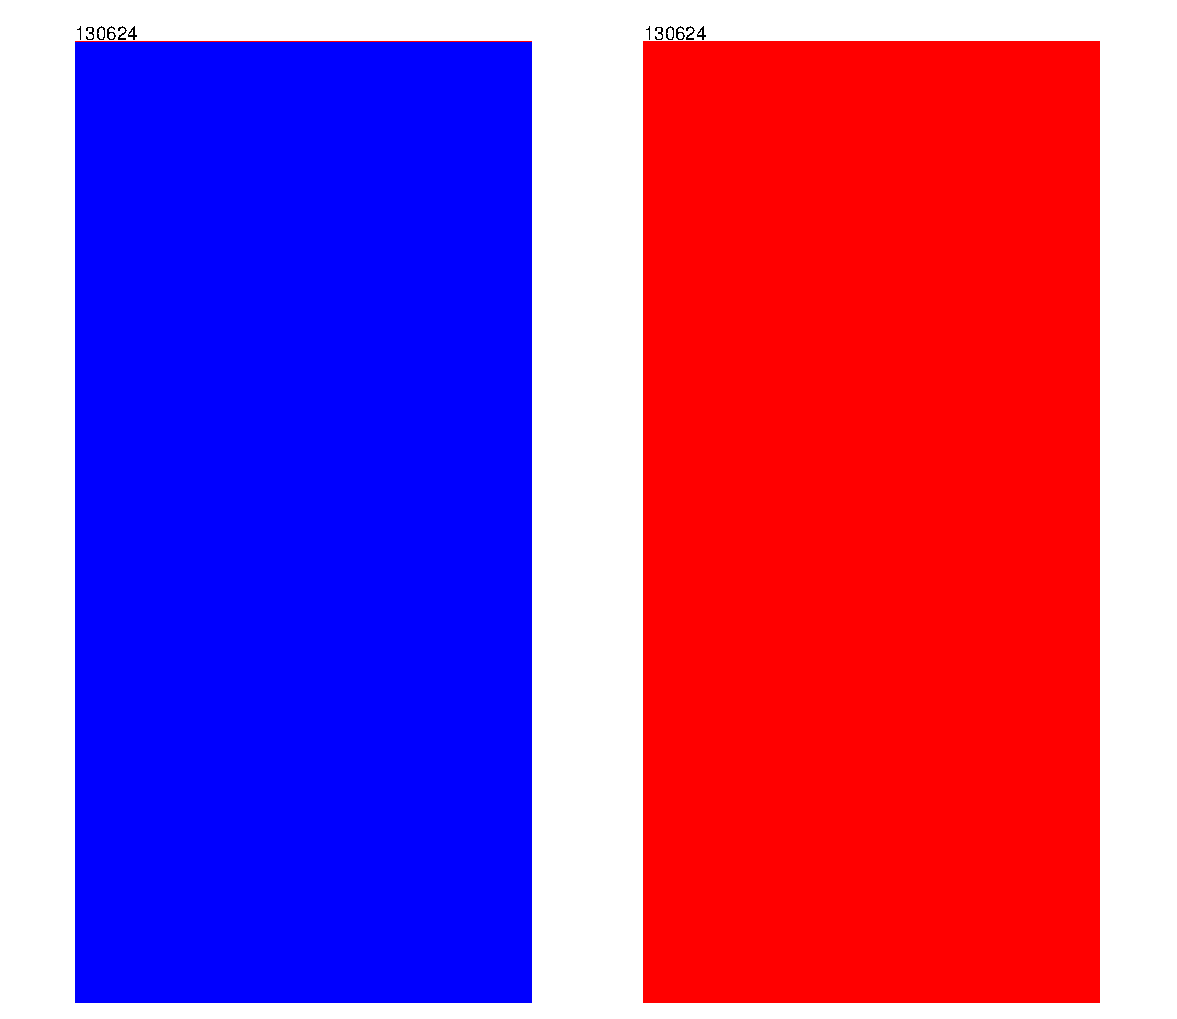
\includegraphics[width=0.46\linewidth]{Figures/l1_f50/set1/active.eps}
} &
\subfloat[gauss 1.]
{
  \label{subfig:l1_f50_set1_gauss1}
  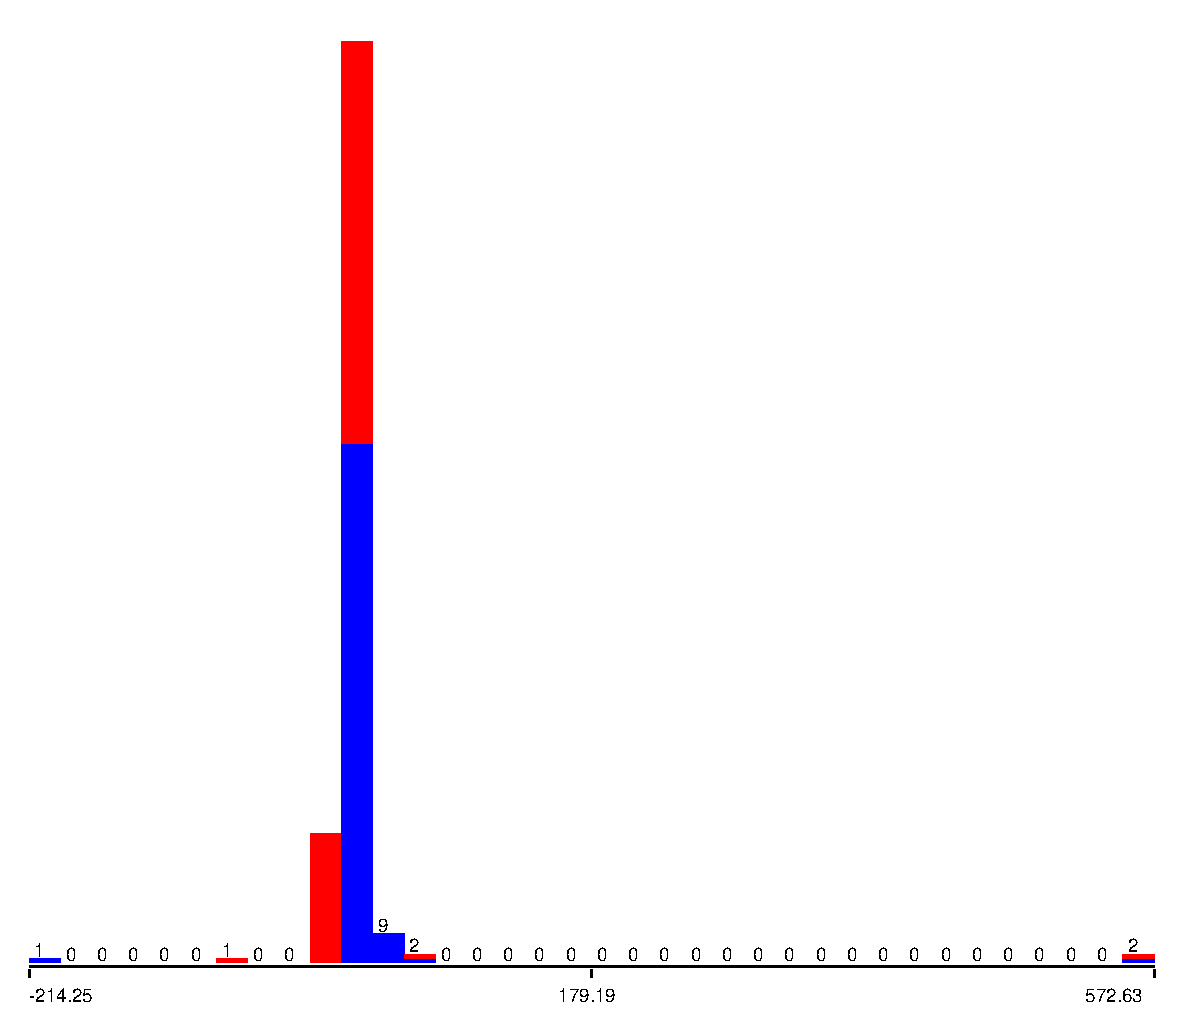
\includegraphics[width=0.46\linewidth]{Figures/l1_f50/set1/gauss1.eps}
} \\
\subfloat[gauss 2.]
{
  \label{subfig:l1_f50_set1_gauss2}
  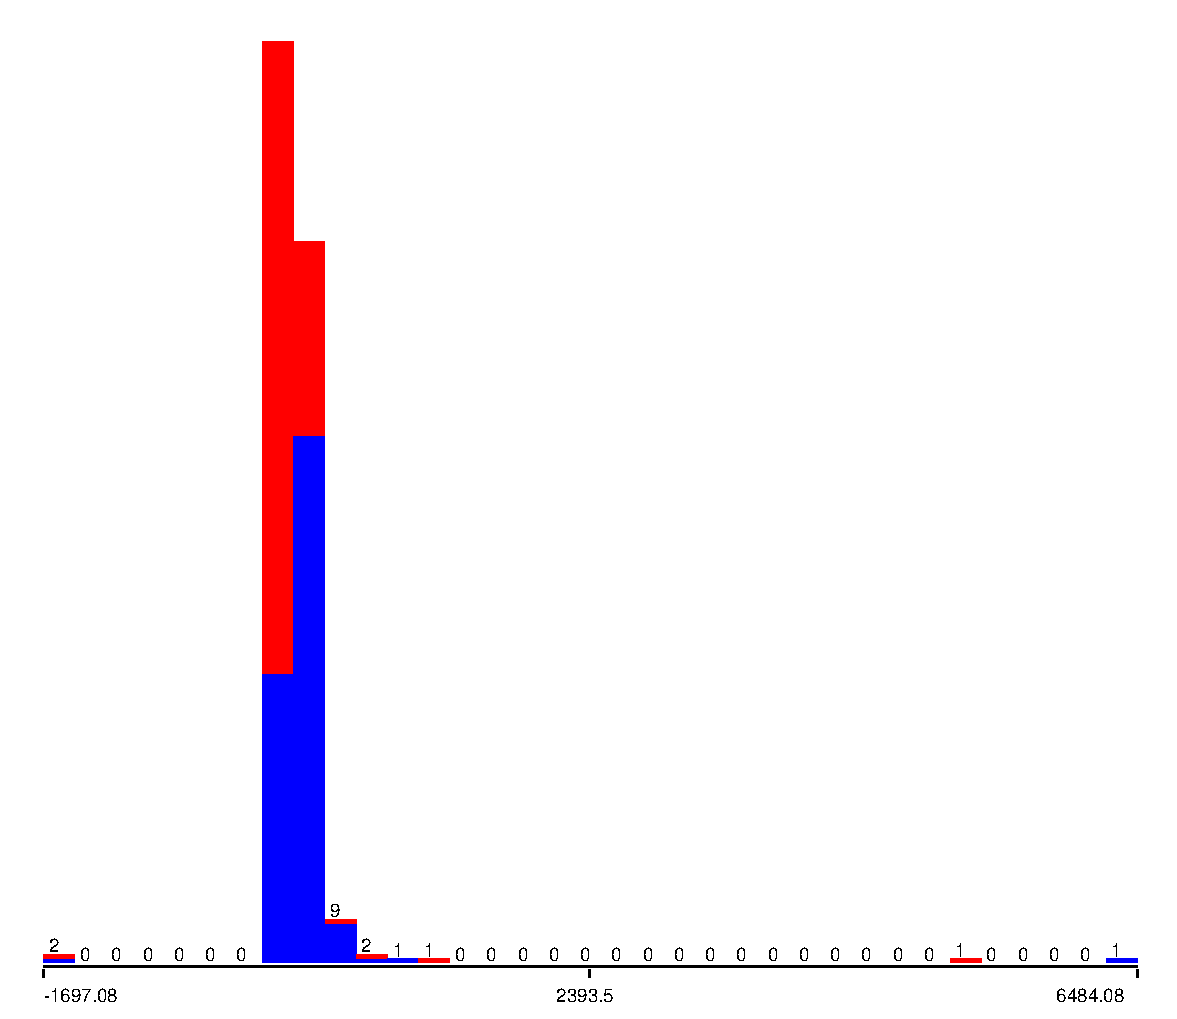
\includegraphics[width=0.46\linewidth]{Figures/l1_f50/set1/gauss2.eps}
} &
\subfloat[repulsion.]
{
  \label{subfig:l1_f50_set1_repulsion}
  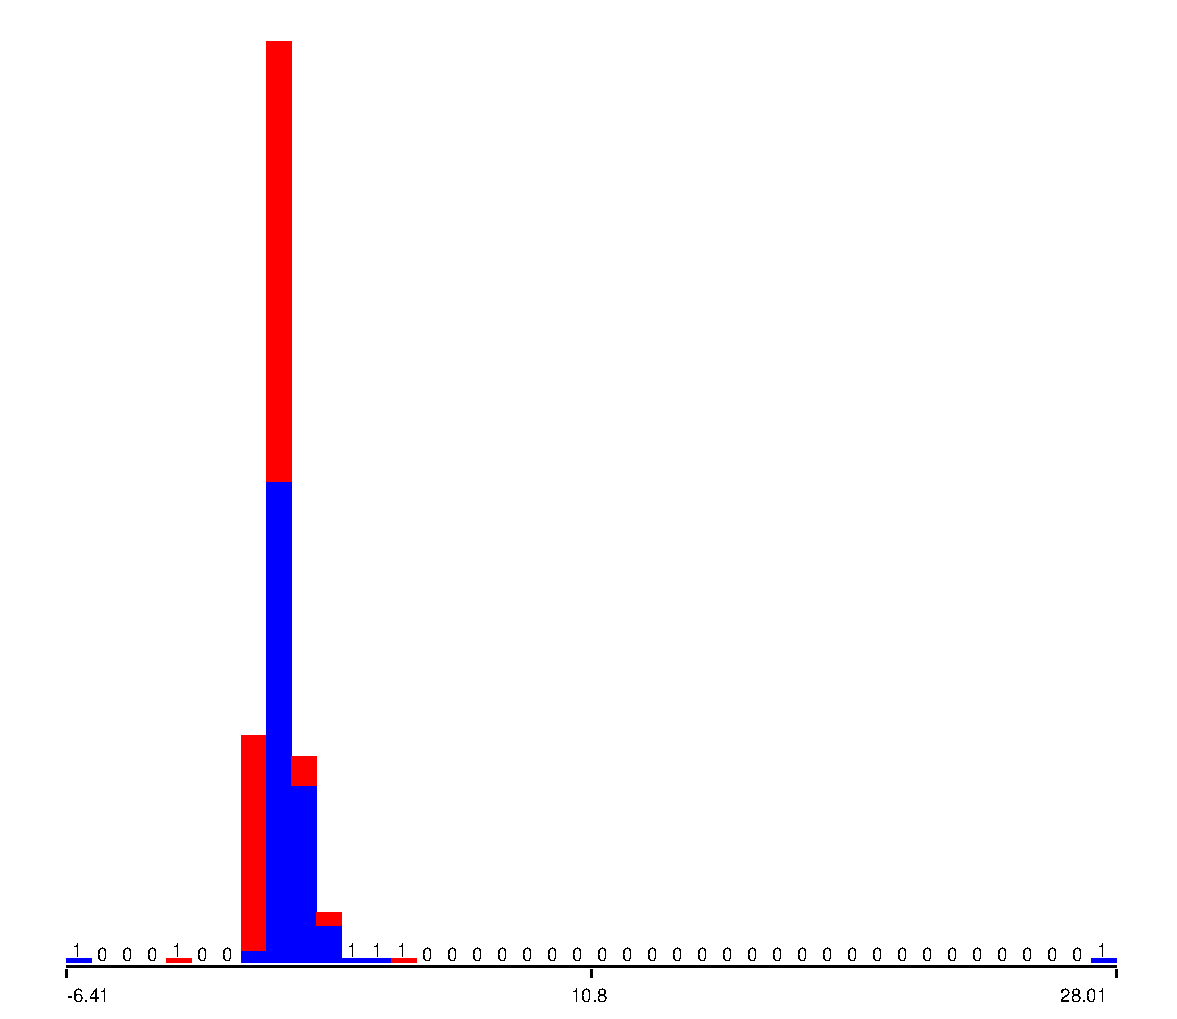
\includegraphics[width=0.46\linewidth]{Figures/l1_f50/set1/repulsion.eps}
} \\
\subfloat[hydrophobic interaction.]
{
  \label{subfig:l1_f50_set1_hydrophobic}
  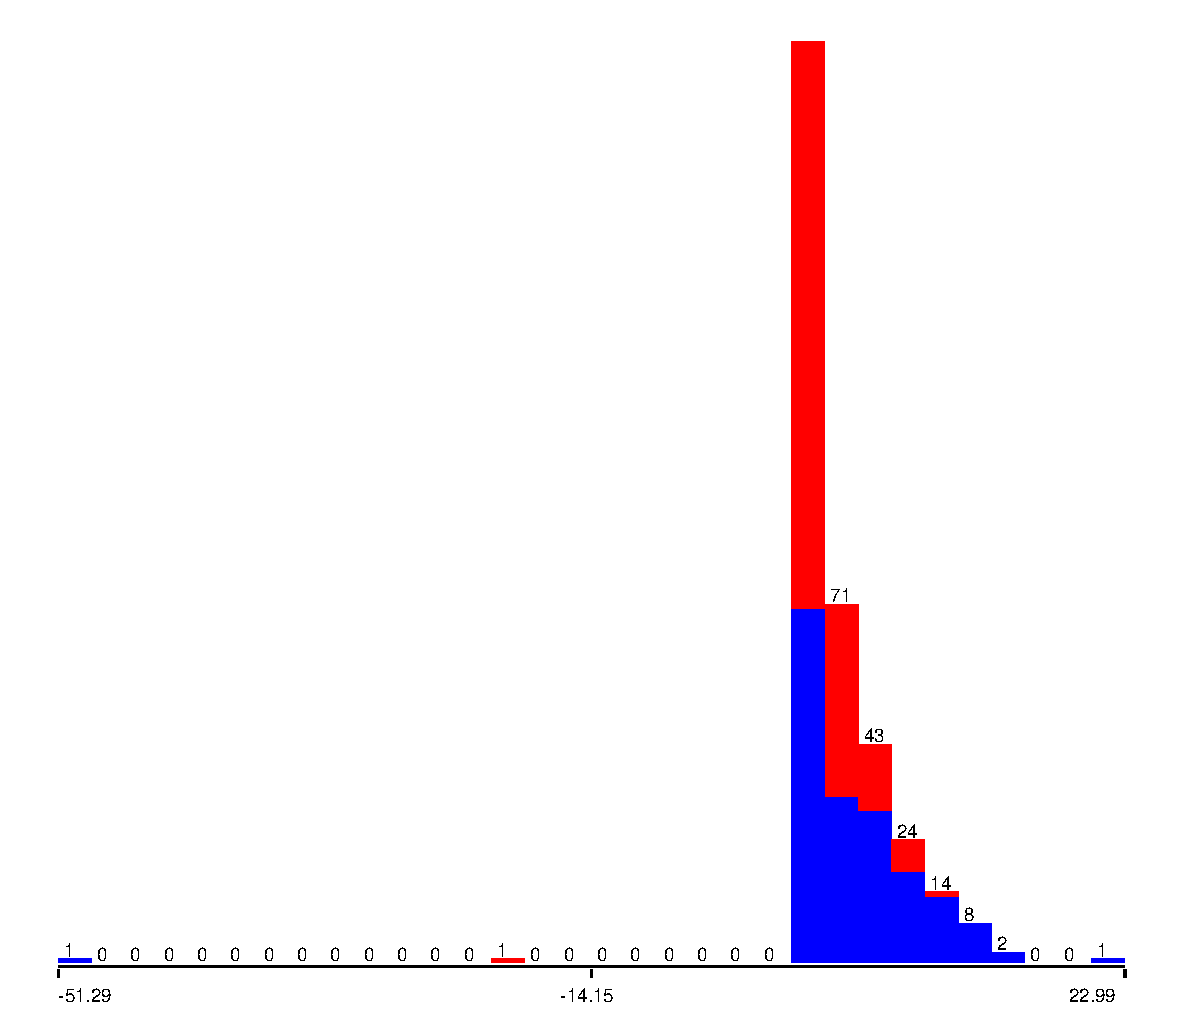
\includegraphics[width=0.46\linewidth]{Figures/l1_f50/set1/hydrophobic.eps}
} &
\subfloat[hydrogen bonding.]
{
  \label{subfig:l1_f50_set1_hydrogenbonding}
  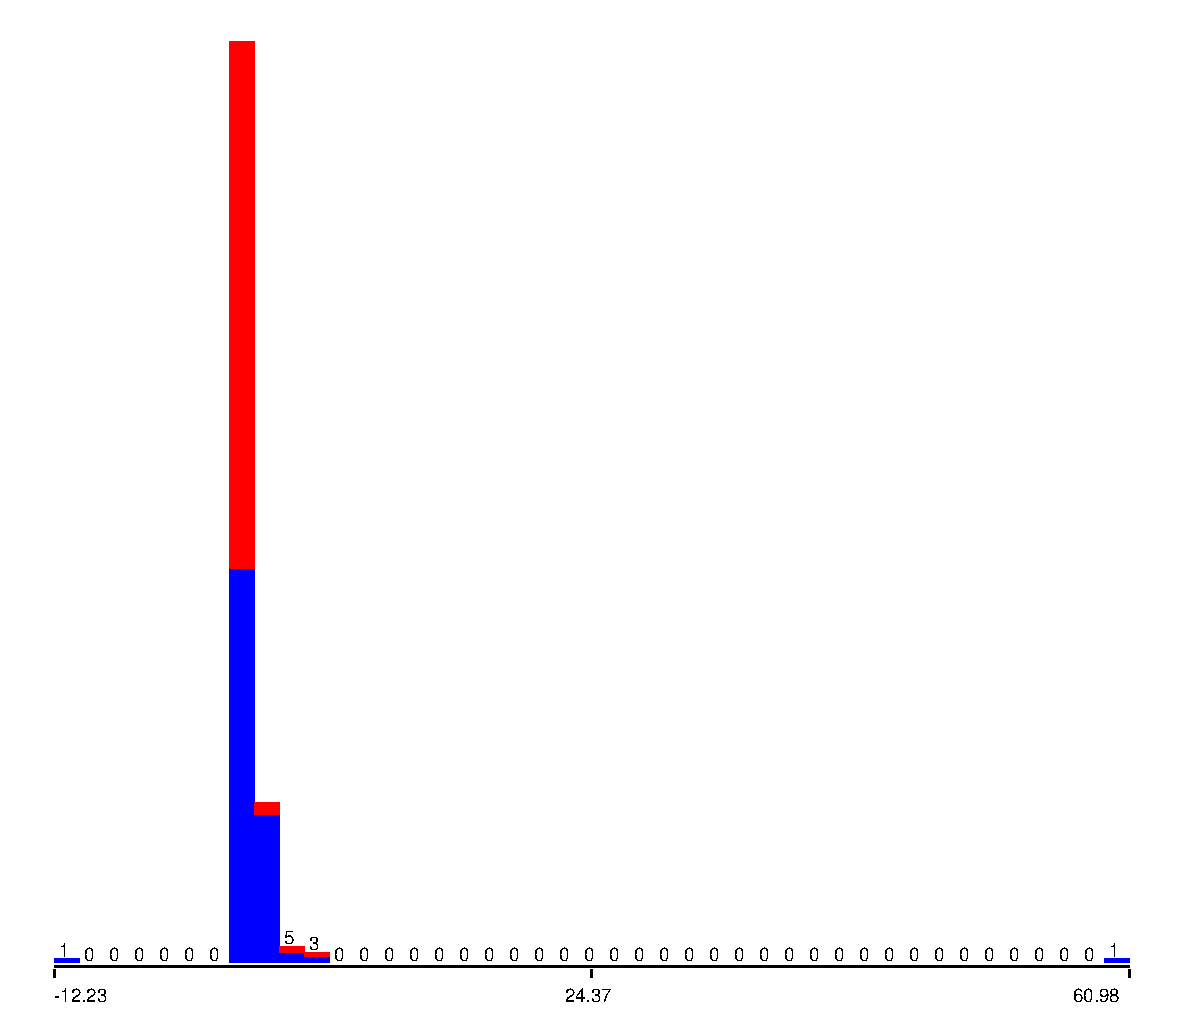
\includegraphics[width=0.46\linewidth]{Figures/l1_f50/set1/hydrogenbonding.eps}
} \\
\end{tabular}
\caption{Distributions of the 5 feature attributes and the binary class attribute of set 1 in case study 1. Class 1 is rendered in blue and class 0 is render in red.}
\label{fig:l1_f50_set1_dists}
\end{figure}

In \citeyear{970}, \Citeauthor{970} developed a program \citep{1316,1317}.

\citep{1263,1264,1319,1084,773,712,377,983,916,304,1040,263,93,1317,1143,705,825,796,940,1082,416,245,289,945,879,1338,1337,1334,402,995,1268,632,1167,1323,1001,357,356,1025,162,1295,1332,1281,908,564,1280,283,473,580,1008,1285,210,1328,1043,1042,878,1315,297,365,518,1157,1197,1139,539,540,537,105,872,793,1090,515,990,824,1267,993,640,548,461,690,675,260,598,978,314,1310,1309,599,937,1174,912,1200,848,1060,1262,1021,492,1333,1133,476,763,964,467,1232,556,311,727,1201,817,986,1118,528,551,1249,1086,1311,1124,1313,563,344,1265,761,1180,691,230,523,322,710,266,262,395,682,895,692,404,292,405,955,602,603,604,1172,1095,1244,547,1005,637,481,332,307,421,1204,355,321,281,927,318,1188,979,764,650,709,1221,725,989,1061,1316,1218,1307,469,1053,1320,1109,804,787,615,233,427,331,889,738,441,1223,1229,930,857,960,999,171,1051,466,954,977,1287,378,1127,693,947,1076,327,1077,1329,997,1208,605,1243,870,987,846,1093,550,549,1110,1146,617,1116,590,661,757,495,701,897,470,648,1228,1245,480,1018,1279,373,721,1239,1242,741,583,890,438,694,1288,1017,1132,400,1096,1209,336,1032,1010,505,1277,1091,486,478,1234,948,949,812,1107,302,552,288,329,325,116,1308,381,924,858,684,873,781,606,667,434,1192,992,273,1100,1147,823,312,865,254,1013,967,272,256,1114,1079,287,1193,1314,487,491,726,291,360,982,534,941,944,1278,462,1298,1282,1270,856,613,502,407,337,353,1080,1292,1312,841,663,1138,1300,962,1011,1236,1136,517,1134,379,496,87,579,833,926,966,435,428,567,1038,1220,784,770,1211,282,533,532,557,1178,1205,743,276,315,88,299,359,1074,1049,1057,1067,1066,891,1187,730,1119,679,520,1293,922,524,204,202,203,1087,906,391,236,585,933,903,914,188,380,1023,301,956,704,1247,115,896,424,317,414,819,1191,797,483,565,608,482,538,1104,1226,792,280,309,686,931,932,1150,1271,1045,1225,394,472,1089,484,1128,593,610,779,607,1039,794,724,961,774,1162,270,805,452,996,1069,1101,1068,1160,894,1155,90,1007,769,910,745,368,714,562,1222,577,450,951,559,902,1130,183,1261,853,386,348,658,91,1121,296,1037,277,1129,303,1020,673,1305,449,251,1153,594,869,425,766,963,695,566,1301,248,974,780,561,859,1024,971,290,750,970,1171,1048,831,1083,1181,611,799,168,167,169,828,1064,1272,1207,835,1166,519,446,374,887,849,659,189,1237,1269,418,542,1149,1148,1035,760,729,1112,795,867,881,330,938,1003,911,1135,443,854,347,345,871,814,165,860,1002,1165,436,1212,772,762,464,366,300,278,1071,349,735,1117,939,791,811,578,1097,1227,584,408,493,844,861,1321,976,597,596,920,506,601,664,925,1156,991,512,535,1294,1030,717,1235,474,1185,591,403,1088,1189,1176,1161,423,1231,1144,998,876,771,1016,1120,362,786,444,782,959,1175,410,1103,1141,1031,333,968,328,655,571,731,293,375,1194,850,432,696,984,929,1246,827,893,1092,1065,1078,716,734,969,119,965,1182,883,1224,728,546,855,1199,980,335,1115,384,159,504,921,440,1219,1324,471,572,711,1125,367,1303,754,1041,429,308,209,498,923,560,1137,905,525,1206,909,439,840,943,672,981,261,574,320,163,1186,697,454,880,242,739,1050,334,431,1290,1327,636,182,396,747,1081,411,422,186,816,419,707,839,862,1276,868,1098,1094,1026,1158,1177,626,733,1250,788,785,1202,830,676,1111,268,269,543,1169,1306,123,1009,390,1006,455,363,1170,588,1331,522,677,813,884,1142,1164,129,1113,181,609,600,975,1046,1284,746,415,326,789,845,285,1233,713,97,1286,666,1304,1168,231,806,904,284,759,521,1028,1000,586,1085,680,1213,1322,1326,815,1198,350,1070,433,581,1108,453,1173,776,832,685,843,448,808,503,744,698,748,740,286,426,722,723,958,900,1184,1154,838,442,1123,1015,915,809,445,864,587,1075,752,973,1289,351,458,1106,829,576,338,699,935,413,687,294,346,742,341,1012,187,1105,279,393,1302,211,1036,936,1131,267,595,490,899,117,323,821,387,688,994,1291,1183,1151,851,399,1054,1179,826,1214,985,477,1248,1027,185,456,736,1159,120,479,886,901,888,485,382,1217,1299,1044,1073,1072,264,1099,247,863,536,531,612,1019,401,972,389,305,950,801,529,530,342,118,343,573,569,526,1210,175,1230,934,1274,681,582,1058,1163,385,810,1052,96,952,802,1238,370,371,928,618,820,275,274,1145,1266,671,1216,570,751,383,1297,1055,1014,803,372,164,1122,758,706,1034,1140,837,1059,575,463,875,885,917,1063,913,919,1283,749,1126,1203,907,376,1241,516,352,866,720,475,489,669,643,614,1275,398,988,1325,775,652,1296,437,1335,392,1056,777}

\bibliographystyle{unsrtnat}
\bibliography{../refworks}

\end{document}

